\subsubsection*{一、选择题}
\setcounter{problemname}{0}

\begin{problem}
	关于优秀设计,以下哪个描述是正确的?
	\uline{C}    
    \vspace{-0.8em}
    \begin{multicols}{2}
        \begin{enumerate}[label=\Alph*.]
            \item 优秀的设计就是很酷的图形
            \item 优秀的设计是常识
            \item 优秀设计源于将用户引入设计中的迭代过程
            \item 优秀设计可能来自于最后对用户界面的修改
        \end{enumerate}
    \end{multicols}
    \vspace{-1em}
\end{problem}



\begin{problem}
	以下描述正确的是:
	\uline{C}    
    \vspace{-0.8em}
    \begin{multicols}{2}
        \begin{enumerate}[label=\Alph*.]
            \item 人机交互只关注软件的可用性
            \item 人机交互就是用户界面设计
            \item “以用户为中心”是交互设计的主要方法
            \item 人机交互只需关注软件设计,不需要关注用户
        \end{enumerate}
    \end{multicols}
    \vspace{-1em}
\end{problem}



\begin{problem}
	为了达到人机交互的设计目标,产品经理和开发人员需要了解以下哪方面的内容:
	\uline{D}    
    \vspace{-0.8em}
    \begin{multicols}{4}
        \begin{enumerate}[label=\Alph*.]
            \item 用户
            \item 任务
            \item 系统的应用环境
            \item 以上全都对
        \end{enumerate}
    \end{multicols}
    \vspace{-1em}
\end{problem}



\begin{problem}
	WYSIWYG 代表的是
	\uline{B}    
    \vspace{-0.8em}
    \begin{multicols}{2}
        \begin{enumerate}[label=\Alph*.]
            \item Where you see is where you get
            \item What you see is what you get
            \item When you see is when you get
            \item Who you see is who you get
        \end{enumerate}
    \end{multicols}
    \vspace{-1em}
\end{problem}



\begin{problem}
	不同专家提出的设计原则之间有密切的关系,如 Ben Shneiderman 提出的八条黄金规则中有一条是“支持内部操作点”,它与 Jcob Nielsen 提出的十条启发式规则中的哪一条对应?
	\uline{C}    
    \vspace{-0.8em}
    \begin{multicols}{2}
        \begin{enumerate}[label=\Alph*.]
            \item 依赖识别而非记忆
            \item  一致性和标准化
            \item 用户享有控制权和自主权
            \item 使用的灵活性和高效
        \end{enumerate}
    \end{multicols}
    \vspace{-1em}
\end{problem}



\begin{problem}
	以下两个网页的主要区别在于:
	\uline{C}
    \begin{figure}[H]
        \setcounter{subfigure}{0}
        \centering
        \vspace{-1em}	
        \subfloat{
        \begin{minipage}[t]{0.44\linewidth}
        \centering
        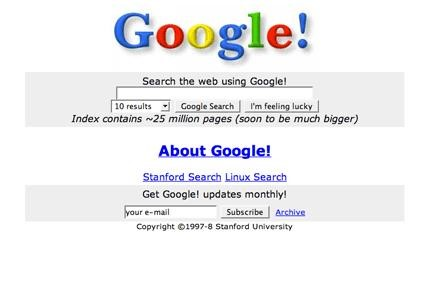
\includegraphics[width=0.97\linewidth]{2.3.1}
        \end{minipage}
        }
        \hfill
        \subfloat{
        \begin{minipage}[t]{0.5\linewidth}
        \centering
        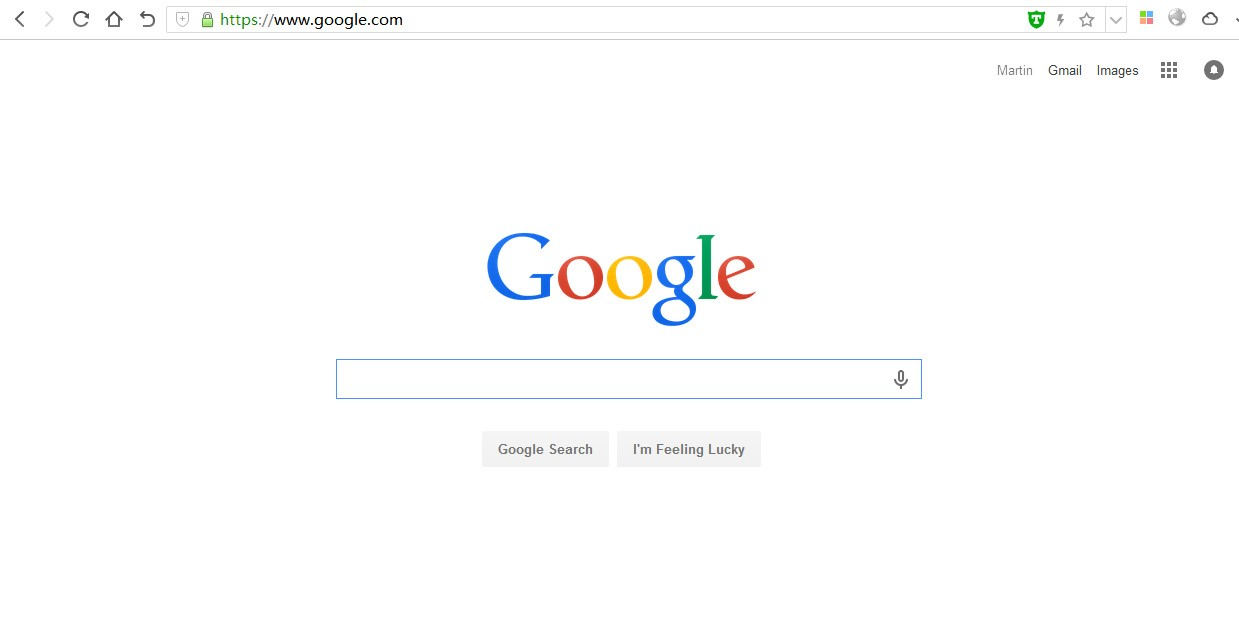
\includegraphics[width=0.97\linewidth]{2.3.2}
        \end{minipage}
        }
        \vspace{-1em}
    \end{figure}
    \vspace{-4em}
    \begin{multicols}{2}
        \begin{enumerate}[label=\Alph*.]
            \item 背景颜色
            \item 第一个网站提供了对结果数量的控制
            \item 第二个网站只包含必要的UI组件
            \item 第二个网站的配色方案更优
        \end{enumerate}
    \end{multicols}
    \vspace{-1em}
\end{problem}



\begin{problem}
	以下关于短时记忆描述正确的是:
	\uline{A}    
    \vspace{-0.8em}
    \begin{multicols}{2}
        \begin{enumerate}[label=\Alph*.]
            \item 短时记忆的容量是有限的
            \item 短时记忆的容量是无限的
            \item 短时记忆的容量为零
            \item 短时记忆的容量很大,但容量有限
        \end{enumerate}
    \end{multicols}
    \vspace{-1em}
\end{problem}



\begin{problem}
	假设需要判断某应用程序的配色方案是否恰当。对于该测试任务,您将使用:
	\uline{B}    
    \vspace{-0.8em}
    \begin{multicols}{2}
        \begin{enumerate}[label=\Alph*.]
            \item  低保真模型
            \item  高保真模型
        \end{enumerate}
    \end{multicols}
    \vspace{-1em}
\end{problem}



\begin{problem}
	原型阶段跟在哪一个开发阶段的后面?
	\uline{C}    
    \vspace{-0.8em}
    \begin{multicols}{4}
        \begin{enumerate}[label=\Alph*.]
            \item 评估
            \item 构建应用程序
            \item 理解用户需要
            \item 以上都不对
        \end{enumerate}
    \end{multicols}
    \vspace{-1em}
\end{problem}



\begin{problem}
	``人物角色不是特定于上下文的,所以它可以很容易地被重复使用”,该表述是
	\uline{B}    
    \vspace{-0.8em}
    \begin{multicols}{2}
        \begin{enumerate}[label=\Alph*.]
            \item 正确的
            \item 错误的
        \end{enumerate}
    \end{multicols}
    \vspace{-1em}
\end{problem}



\begin{problem}
	以用户为中心的设计方法很重要,这是因为:
	\uline{B}    
    \vspace{-0.8em}
    \begin{multicols}{2}
        \begin{enumerate}[label=\Alph*.]
            \item 用户需要被教导如何使用设计产品
            \item 系统设计应该对用户足够直观
            \item 系统设计应特别迎合使用者的需要
            \item 在进行设计时,有必要了解用户所处的环境
        \end{enumerate}
    \end{multicols}
    \vspace{-1em}
\end{problem}



\begin{problem}
	现实世界中对事务的控制及其影响之间的关系指的是:
	\uline{C}    
    \vspace{-0.8em}
    \begin{multicols}{3}
        \begin{enumerate}[label=\Alph*.]
            \item 可见性 Visibility
            \item 功能可见性 Affordance
            \item 映射 Mapping
        \end{enumerate}
    \end{multicols}
    \vspace{-1em}
\end{problem}



\begin{problem}
	GOMS 表示的是:
	\uline{A}    
    \vspace{-0.8em}
    \begin{multicols}{2}
        \begin{enumerate}[label=\Alph*.]
            \item  Goals, operation, methods and selection rules
            \item  Goals, objects, models and selection rules
            \item  Goals, operations, methods and state rules
            \item  Goals, operations, models and state rules
        \end{enumerate}
    \end{multicols}
    \vspace{-1em}
\end{problem}



\begin{problem}
	为探索小孩子们在一起是如何交谈的,并调查一种新型产品是否能帮助他们更积极地参与其中,可使用如下哪种技术:
	\uline{B}    
    \vspace{-0.8em}
    \begin{multicols}{4}
        \begin{enumerate}[label=\Alph*.]
            \item 可用性测试
            \item 实地研究
            \item 预测性评估
            \item DECIDE 框架
        \end{enumerate}
    \end{multicols}
    \vspace{-1em}
\end{problem}



\begin{problem}
	关于启发式评估,以下论证正确的是:
	\uline{A}    
    \begin{enumerate}[label=\Alph*.]
        \item 启发式评估是一种基于专家的评估方法
        \item 专家应用启发式评估时,会从自身使用经验出发对界面进行判断
        \item 启发式评估的结果只有界面中潜在的可用性问题列表
        \item 当界面元素存在多个可用性问题时,只需列举其中一个问题即可
    \end{enumerate}
\end{problem}

